%!TeX root =  ../../thesis.tex

\section{Arduino IDE}
Jako vývojové prostředí používám oficiální Arduino IDE, což mi zaručuje kompatibilitu s jednodeskovým počítačem Arduino a také je crossplatformní, což jako uživatel Linuxu vítám. Součástí IDE jsou také standardní knihovny pro Arduino, tudíž není ani důvod používat jiné IDE pro práci s Arduinem.

\begin{figure}[h]
	\centering
	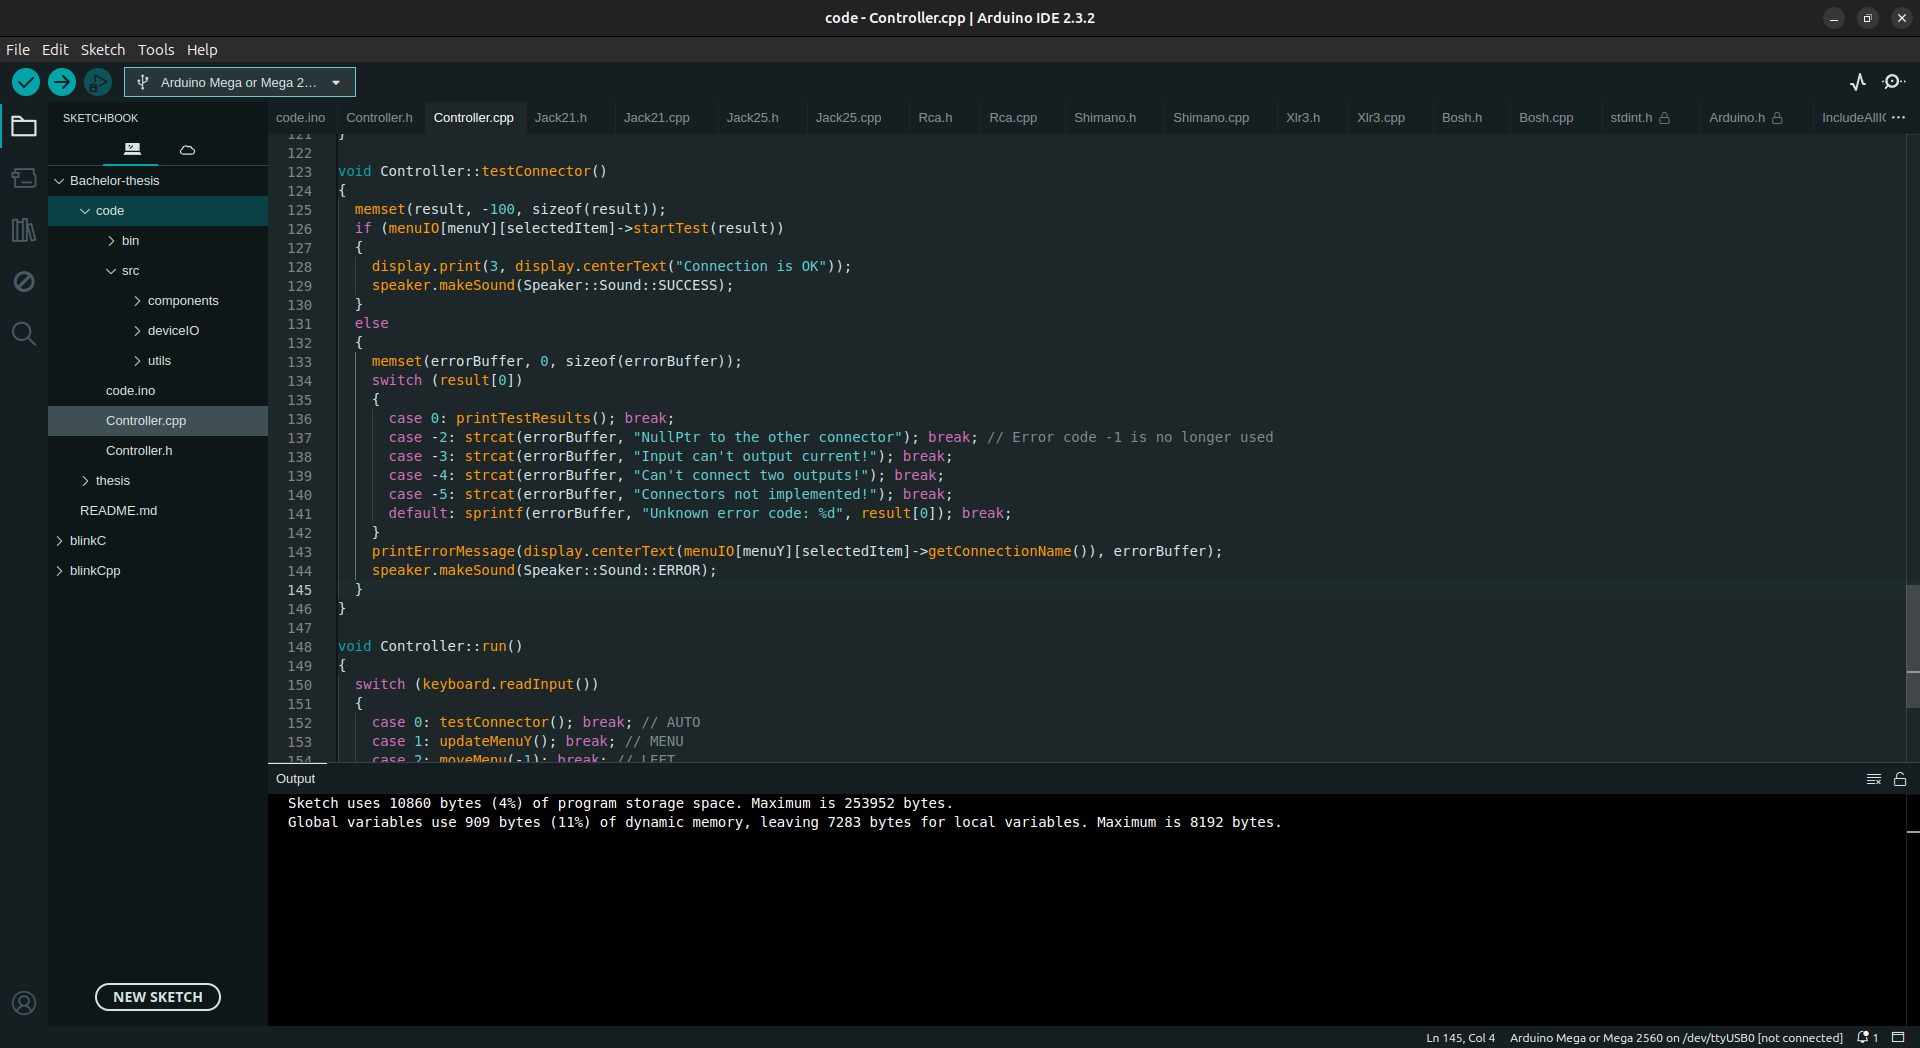
\includegraphics[width=\textwidth]{pictures/arduinoIDE.png}
    	\caption{Vývojové prostřední Arduino}
   	\label{fig:arduinoIDE}
\end{figure}
\newpage
Na obrázku \ref{fig:arduinoIDE} je vývojové prostředí Arduino, můžeme si všimnout, že ve spodní části je konzole s výstupem, nyní tam je výsledek kompilace programu, dále vpravo je struktura projektu. Arduino IDE vyžaduje pevnou strukturu, kód, který nebude v hlavní složce, musí být ve složce “src”. Hlavní soubor se musí jmenovat jako složka ve které je umístěn a musí být typu “.ino”, v tomto souboru je kód v jazyce Arduino a obsahuje vždy minimálně dvě metody.\\
Metodu “setup()” a metodu “loop()”, metoda “setup()” slouží k inicializaci zařízení a metoda “loop()” obsahuje kód, který je vykonáván mikrokontrolérem ve smyčce, dokud není nějakým způsobem přerušen.

\subsection{Programovací jazyk}
Arduino se dá v základu programovat pomocí jazyku Arduino, který je založená na jazyce AVR-C, nebo také v C/C++. Já jej budu programovat v jazyce C++, jelikož s ním mám zkušenost a objektový přístup ulehčí implementaci konektorů a jejich následnému testování. Ačkoliv se pro tyto účely používá spíše jazyk C, tak pro potřeby navrhovaného zařízení by použití jazyka C nepřineslo žádnou znatelnou výhodu oproti C++.